%!TEX root = ../main.tex

To sum up, \textit{\gls{pem} identification} is a common paradigm for finding suitable models from data, based on prediction theory.

We have to move from stochastic models (ARMAX models) of type: 

$$
\Mc(\theta):\quad
y(t) = \frac{B(z,\theta)}{A(z,\theta)} u(t-d) +\ \frac{C(z,\theta)}{A(z,\theta)} e(t) ,\ e(t)\sim \WN(0,\lambda ^{2})
$$

to models in prediction form, i.e. the optimal predictors obtained through the theory we developed. In particular, we can focus on the \textbf{one-step predictor} already introduced:

$$
\hat{\Mc}(\theta):\quad
\hat{y}(t\mid t-1) = \frac{B(z,\theta) E(z,\theta) \ }{C(z,\theta)} u(t-d) + \frac{F(z,\theta)}{C(z,\theta)} y(t-1)
$$

The predictor has a different structure: while $ \Mc(\theta)$ is fed by a \gls{wn} and an input $u$, the predictor $\hat{\Mc}(\theta)$ is fed by measurements of $u$ and $y$ and returns the predicted future values of output, \textbf{there isn't a \gls{wn}}. The predictor model is returning the predicted values for \textit{that} realization of input and output.

\begin{figure}[htpb]
	\centering
	\begin{subfigure}{.5\textwidth}
		\centering
		\begin{tikzpicture}
			% place nodes
			\node [block] (m) at (0,0) {$\mathcal{M}(\vartheta)$};
			% connect nodes
			\draw [stealth-] (m.west) -- ++(-2,0) node[midway,above] {$u(t)$};
			\draw [stealth-] (m.north) -- ++(0,1) node[midway,right] {$e(t)$};
			\draw [-stealth] (m.east) -- ++(2,0) node[midway,above] {$y(t)$};
		\end{tikzpicture}
	\end{subfigure}%
	\begin{subfigure}{.5\textwidth}
		\centering
		\begin{tikzpicture}
			% place nodes
			\node [block] (m) at (0,0) {$\hat{\mathcal{M}}(\vartheta)$};
			% connect nodes
			\draw [stealth-] ([shift={(0, 0.2)}]m.west) -- ++(-2,0) node[midway,above] {$u(t-d)$};
			\draw [stealth-] ([shift={(0,-0.2)}]m.west) -- ++(-2,0) node[midway,below] {$y(t-1)$};
			\draw [-stealth] (m.east) -- ++(2,0) node[midway,above] {$\hat{y}(t\mid t-1)$};
		\end{tikzpicture}
	\end{subfigure}
\end{figure}
\FloatBarrier

The idea is that, when dealing with a real system, the values of $u$ and $y$ from time $t=1,\ldots,n$ can be collected, subsequently taking the predictor (introducing proper delays $ z^{-1}$) and feeding it with the measurement of $u$ and $y$ collected during the experiment. Then, the output of the predictor $\hat{\Mc}(\theta $) can be used to construct the value of the \textbf{prediction error} $ \varepsilon $. 
\begin{figure}[htpb]
	\centering
	\begin{tikzpicture}

		\node (origin) at (0,0) {};
		\node[cloud, draw, right=1.5cm of origin,
		    minimum width = 3cm,
	        minimum height = 2cm] (c) {$S$};
		
		\draw[-stealth] (origin.east) -- (c.west)
		    node[midway,above] {$u(t)$}
		    node[midway,below] {$ \begin{array}{c} \bar{u}(1)\\ \vdots \\ \bar{u}(n) \end{array}$}
		    node[near end] (u) {}
		    node[at end] (inputR) {};
		    
		\node[sum,below right = 1cm and 6cm of c.east] (s) {};
		\node[draw,
		minimum width=2cm,
	    minimum height=1.5cm,below left = 1cm and 1cm of s.center] (M) {$\hat{\mathcal{M}}(\theta)$};
	    
		\node[block,above left = 0.1cm and 1cm of M.west] (z1) {$z^{-1}$};
		\node[block,below left = 0.1cm and 1cm of M.west] (z2) {$z^{-1}$};
		
		\draw[-stealth] (c.east)-|(s.north)
		    node[pos=0.05] (fed) {}
		    node[near start,above] {$y(t)$}
		    node[near start,below] {$ \begin{array}{c}\bar{y}(1)\\ \vdots \\ \bar{y}(n)\end{array}$}
		    node[very near end, right] {$+$}
		;
		
		\draw[-stealth] (fed.center) |- (z1.west);
		\draw[-stealth]   (u.center) |- (z2.west);
		
		\draw[-stealth] (z1.east) -- ++(1,0);
		\draw[-stealth] (z2.east) -- ++(1,0);
		
		\draw[-stealth] (M.east)-|(s.south)
		    node[midway,right] {$\hat{y}(t\mid t-1,\theta)$}
		    node[very near end, right] {$-$}
		;
		
		\draw[-stealth] (s.east) -- ++(3,0)
		    node[midway,above]{$\varepsilon (t\mid t-1,\theta)$}
		    node[very near end] (startMin) {}
		;

		\draw[dashed,-stealth]
		    (startMin) -- ++(0,-3) -- ++(-5,0) 
		    node[midway,above]{$\min$}
		    -- ++(0,0.5)
		;
	\end{tikzpicture}
	\caption{The \gls{pem} identification scheme.}
\end{figure}
% \FloatBarrier

\begin{center}

\begin{tabular}{ccccc}
\toprule 
 $t$ & $u$ & $y$ & $ \hat{y}$ & $ \varepsilon $ \\
\midrule 
 $1$ & $ u(1)$ & $ y(1)$ & $ \hat{y}(1\mid 0)$ & $ \varepsilon (1\mid 0,\theta)$ \\
$2$ & $ u(2)$ & $ y(2)$ & $ \hat{y}(2\mid 1)$ & $ \varepsilon (2\mid 1,\theta)$ \\
$ \vdots $ & $ \vdots $ & $ \vdots $ & $ \vdots $ & $ \vdots $ \\
$n$ & $ u(n)$ & $ y(n)$ & $ \hat{y}(n\mid n-1)$ & $ \varepsilon (n\mid n-1,\theta)$ \\
 \bottomrule
\end{tabular}
\end{center}

All the values $ \hat{y} ,\ \varepsilon $ depend on the chosen $ \theta $. By inspecting the value of $ \varepsilon $, $ \theta $ can be tuned to make the prediction error as small as possible through a minimization process.

\textbf{We want to choose $\hat{\theta}_{N}$ that minimizes the prediction error.}

We have to introduce a metric to quantify the error. We define a \textbf{cost function:} 
\begin{equation*}
	\boxed{J_{N}(\theta) =\frac{1}{N}\sum _{i=1}^{N}(y(i) -\hat{y}(i\mid i-1,\theta))^{2} =\frac{1}{N}\sum _{i=1}^{N} \varepsilon (i\mid i-1,\theta)^{2}}
\end{equation*}
also known as \textbf{\gls{pem} minimization cost}, which can be interpreted as the \emph{empirical variance} of the prediction error over the collected data. Then:
\[
	\boxed{\hat{\theta }_{N} =\underset{\theta \in \Theta}{\argmin} J_{N}(\theta) =\underset{\theta \in \Theta}{\argmin}\frac{1}{N}\sum _{i=1}^{N} \varepsilon (i\mid i-1,\theta)^{2}}
\]

\subsection{Estimation of \texorpdfstring{$\lambda$}{lambda}}

$ \hat{\Mc}(\theta)$ depends only on $ \theta $ and the minimization of $J_{N}(\theta)$ returns only the best estimate for $\theta$, the part of the model that we need in order to reconstruct the predictor.

However, if we're interested in the description of the complete ARMA process, also $\lambda^{2}$ has to be estimated. 
\begin{equation*}
	\boxed{\hat{\lambda }_{N}^{2} =J_{N}(\hat{\theta }_{N}) =\frac{1}{N}\sum _{i=1}^{N} \varepsilon (i\mid i-1,\hat{\theta }_{N})^{2}}
\end{equation*}
The proposed estimate is the \textbf{empirical variance} of the prediction error for the optimal model. The idea behind the formula is simple: suppose $ S\in \Mc $ (i.e. our model class is rich enough to describe perfectly the true mechanism by which $y$ is generated) and $\hat{\theta }_{N}$ is so good that $\Mc(\hat{\theta }_{N}) =S$ (i.e. the information collected is enough to unveil $S$).

Since $ S\in \Mc \Longrightarrow S$ is an ARMAX process. Thus, there is a white noise $ \xi (t) \sim \WN(0,\lambda ^{2})$ in the real world that generates $y$. Then $ \hat{y}(t\mid t-1,\hat{\theta }_{N})$ is the optimal predictor not only for the model, but also for the system $S$. Most importantly
\begin{equation*}
\varepsilon (t\mid t-1,\hat{\theta }_{N}) =\xi (t)
\end{equation*}
the one-step prediction error in optimal prediction \textit{is} the \gls{wn} in the system. It makes sense to approximate the true variance by means of an empirical variance:
\begin{gather*}
\lambda ^{2} =\mathbb{E}\left[ \xi (t)^{2}\right] =\mathbb{E}[ \varepsilon (t\mid t-1,\hat{\theta }_{N})^2]\\
\hat{\lambda }_{N}^{2} =J_{N}(\hat{\theta }_{N}) =\frac{1}{N}\sum _{i=1}^{N} \varepsilon (i\mid i-1,\hat{\theta }_{N})^{2}
\end{gather*}

\subsection{Least Squares Identification (AR/ARX processes)}
Now that we have our model, we need to study its computational aspect: how can the cost function be minimized with respect to $ \theta ?$

In general $ J_{N}(\theta)$ is a very complicated and non-convex function of $ \theta $, with local minima and often without analytical or explicit expression. However, the subset of AR/ARX models, with good descriptive capabilities, has a quadratic cost function which can be explicitly minimized.

In this case \gls{pem} Identification takes the name of \textbf{Least Squares Identification.}

Given a generic ARX model
\begin{gather*}
y(t) =\frac{B(z,\theta)}{A(z,\theta)} u(t-d) +\frac{1}{A(z,\theta)} e(t) \qquad e(t) \sim \WN(0,\lambda ^{2})\\
A(z,\theta) =1-a_{1} z^{-1} -\cdots -a_{m} z^{-m}\\
B(z,\theta) =b_{0} +b_{1} z^{-1} +\cdots +b_{p} z^{-p}
\end{gather*}
with the black-box assumptions that we made, theta is the vector of the coefficients
\begin{equation*}
\theta = [ a_{1},\ldots,a_{m},b_{0},b_{1},\ldots,b_{p}]\transpose
\end{equation*}
The recursive equations associated to the model are
\begin{gather*}
A(z,\theta) y(t) =B(t,\theta) u(t-d) +e(t)\\
\left(1-a_{1} z^{1} -\cdots -a_{m} z^{-m}\right) y(t) =\left(b_{0} +b_{1} z^{-1} +\cdots +b_{p} z^{-p}\right) u(t-d) +e(t)\\
\Downarrow \\
y(t) =a_{1} y(t-1) +\cdots +a_{m} y(t-m) +b_{0} u(t-d) +b_{1} u(t-d-1) +\cdots +b_{p} u(t-d-p) +e(t)
\end{gather*}
If we introduce the vector of the regression variables $ \varphi $
\begin{equation*}
\varphi (t) =\begin{bmatrix}
y(t-1)\\
\vdots\\
y(t-m)\\
u(t-d)\\
u(t-d-1)\\
\vdots\\
u(t-d-p)
\end{bmatrix}
\end{equation*}
we can rewrite the recursive equations
\begin{equation*}
	y(t) =\underbrace{\varphi (t)\transpose \theta }_{\substack{\text{predictable}\\\text{at }t-1}} +\underbrace{e(t)}_{\substack{\text{unpredictable}\\\text{at }t-1}}
\end{equation*}
It is now possible to compute the one-step predictor for ARX model easily: we just need to delete the unpredictable part.
\begin{align*}
	\hat{\Mc}(\theta) :\ \hat{y}(t\mid t-1) & =a_{1} y(t-1) +\cdots +a_{m} y(t-m) +b_{0} u(t-d) +\cdots +b_{p} u(t-d-p)\\
	& =\varphi (t)\transpose \theta 
\end{align*}
The predictor is a very simple expression, a linear function of $ \theta $.

The identification cost is quadratic and positive:		
\begin{align*}
J_{N}(\theta) & =\frac{1}{N}\sum _{t=1}^{N}(y(t) -\hat{y}(t\mid t-1,\theta))^{2} & \\
 & =\frac{1}{N}\sum _{t=1}^{N}\left(y(t) -\theta \transpose \varphi (t)\right)^{2} & (\text{quadratic function of} \ \theta) \\
 & \geq \ 0 & \text{(sum of squares)}
\end{align*}


$ \hat{\theta }_{N}$ is the minimum of a quadratic and positive function, and is therefore determined by the first order condition:
\begin{equation*}
\frac{d}{d\theta } J_{N}(\theta) =\begin{bmatrix}
\frac{\partial J_{N}}{\partial a_{1}}(\theta)\\
\vdots \\
\frac{\partial J_{N}}{\partial b_{p}}(\theta)
\end{bmatrix} =0
\end{equation*}
i.e. a system of linear equations whose solutions are all and only minimizers of $ J_{N}(\theta)$.

By substitution:
\begin{align*}
\frac{d}{d\theta } J_{N}(\theta) & =\frac{d}{d\theta }[\frac{1}{N}\sum _{t=1}^{N}\left(y(t) -\theta \transpose \varphi (t)\right)^{2}] & \text{(linearity)}\\
 & =\frac{1}{N}\sum _{t=1}^{N}\frac{d}{d\theta }\left(y(t) -\theta \transpose \varphi (t)\right)^{2} & \\
 & =\frac{1}{N}\sum _{t=1}^{N} 2\left(y(t) -\theta \transpose \varphi (t)\right)\frac{d}{d\theta }\left(y(t) -\theta \transpose \varphi (t)\right) & \frac{d}{d\theta } y(t) =\begin{bmatrix}
0\\
\vdots \\
0
\end{bmatrix}\\
 & =\frac{1}{N}\sum _{t=1}^{N} 2\left(y(t) -\theta \transpose \varphi (t)\right)\frac{d}{d\theta }\left(-\theta \transpose \varphi (t)\right) & \frac{d}{d\theta }\left(-\theta \transpose \varphi (t)\right) =-\varphi (t)\\
 & =\frac{1}{N}\sum _{t=1}^{N} 2\underbrace{\left(y(t) -\varphi (t)\transpose \theta \right)}_{\text{scalar}}\underbrace{(-\varphi (t))}_{\text{column vec}} & \\
 & =\frac{2}{N}\sum _{t=1}^{N} \varphi (t)\left(\varphi (t)\transpose \theta -y(t)\right) & \\
 & =\frac{2}{N}\sum _{t=1}^{N} \varphi (t) \varphi (t)\transpose \theta \ -\frac{2}{N}\sum _{t=1}^{N} \varphi (t) y(t) & 
\end{align*} \ 
Setting $ \frac{d}{d\theta } J_{N}(\theta) =0$	


\begin{align*}
\cancel{\frac{2}{N}}\sum _{t=1}^{N} \varphi (t) \varphi (t)\transpose \theta  & =\cancel{\frac{2}{N}}\sum _{t=1}^{N} \varphi (t) y(t) & \\
\left[\sum _{t=1}^{N} \varphi (t) \varphi (t)\transpose\right] \theta  & =\sum _{t=1}^{N} \varphi (t) y(t) & \text{system of linear eqs in} \ \theta 
\end{align*}
This system of linear equations is commonly referred to as \textbf{Least Squares Normal Equations}. If 
\begin{equation*}
\sum _{t=1}^{N} \varphi (t) \varphi (t)\transpose \ \text{is non-singular}
\end{equation*}
the solution is unique, and $ \hat{\theta }_{N}$ is uniquely determined
\begin{equation*}
\boxed{\hat{\theta }_{N} =\left[\sum _{t=1}^{N} \varphi (t) \varphi (t)\transpose\right]^{-1}\sum _{t=1}^{N} \varphi (t) y(t)}
\end{equation*}
If $ \sum \varphi (t) \varphi (t)\transpose$ is singular, there are infinite solutions: $ \hat{\theta }_{N}$ can be determined by introducing a tie-break rule (e.g. taking the solution with minimum norm). This may happen when many models have the same predictive capability, such as in a redundant model class or in case of uninformative data.

\textbf{Geometric interpretation:}
\begin{equation*}
J_{N}(\theta) =\frac{1}{N}\sum _{t=1}^{N}\left(y(t) -\theta \transpose \varphi (t)\right)^{2}
\end{equation*}
is a paraboloid. The Hessian matrix $ \frac{d^{2}}{d\theta ^{2}} J_{N}(\theta)$ completely characterizes the space of quadratic functions.
\begin{align*}
\frac{d}{d\theta } J_{N}(\theta) & =\frac{2}{N}\sum _{t=1}^{N} \varphi (t) \varphi (t)\transpose \theta \ -\frac{2}{N}\sum _{t=1}^{N} \varphi (t) y(t)\\
\frac{d^{2}}{d\theta ^{2}} J_{N}(\theta) & =\frac{2}{N}\underbrace{\sum _{t=1}^{N} \varphi (t) \varphi (t)\transpose}_{\text{information matrix}}
\end{align*}
The information matrix is positive semi-definite. Indeed, taking a generic vector $x$ and remembering that $x\transpose \varphi (t) =\varphi (t)\transpose x$,
\[
	x\transpose\frac{d^{2}}{d\theta ^{2}} J_{N}(\theta) x = \frac{2}{N} x\transpose\left[\sum _{t=1}^{N} \varphi (t) \varphi (t)\transpose\right] x=\frac{2}{N}\sum _{t=1}^{N}\left(x\transpose \varphi (t)\right)^{2} \geq 0 \quad \forall x\neq 0
\]
$ J_{N}(\theta)$ is a paraboloid with minima:
\begin{figure}[htpb]
	\centering
	\begin{subfigure}{.5\textwidth}
		\centering
		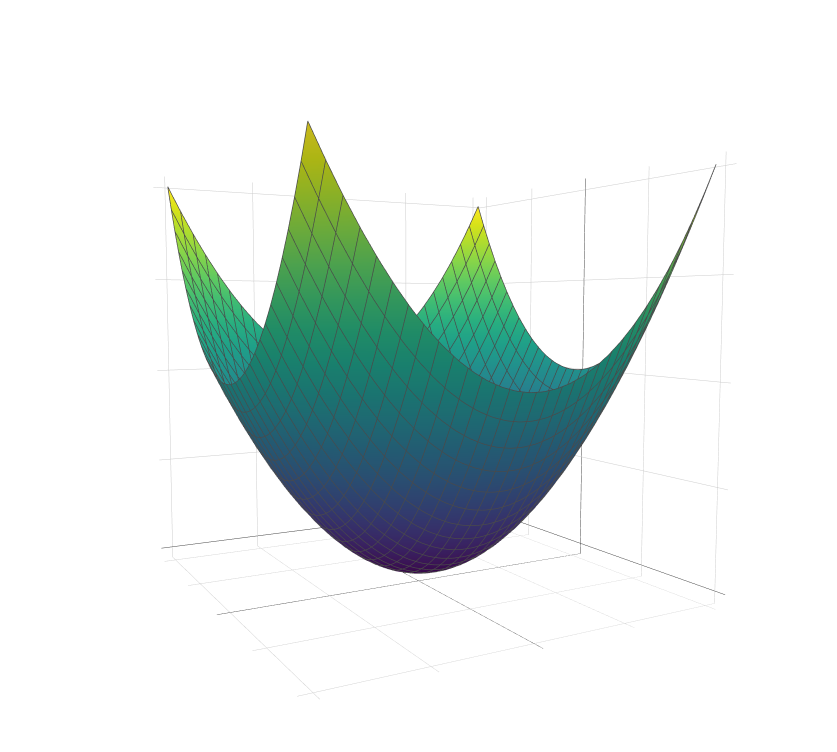
\includegraphics[width=.8\linewidth]{paraboloid-proper}
		\captionof{figure}{Proper paraboloid}
		\label{fig:test1}
	\end{subfigure}%
	\begin{subfigure}{.5\textwidth}
		\centering
		
\includegraphics[width=.8\linewidth]{paraboloid-degenerate}
		\captionof{figure}{Degenerate paraboloid}
		\label{fig:test2}
	\end{subfigure}
\end{figure}
\FloatBarrier
\begin{align*}
\frac{d^{2}}{d\theta ^{2}} J_{N}(\theta) & =\frac{2}{N}\sum _{t=1}^{N} \varphi (t) \varphi (t)\transpose \text{ non-singular (pos. def.)} & \Longrightarrow\quad& \text{proper paraboloid (unique min.)}\\
\frac{d^{2}}{d\theta ^{2}} J_{N}(\theta) & =\frac{2}{N}\sum _{t=1}^{N} \varphi (t) \varphi (t)\transpose \text{ singular} &\Longrightarrow\quad& \text{degenerate paraboloid}
\end{align*}